\documentclass{article}
\usepackage{amsmath}
\usepackage{enumerate}
\usepackage{listings}
\usepackage{moreverb}
\usepackage[margin=1in]{geometry}
\usepackage{graphicx}
\usepackage{dsfont}
\title{STA 360: Assignment 10}
\author{Michael Lin}

\begin{document}
\maketitle
\begin{enumerate}
\item See appendix for procedure and result of hypothesis testing.

\item This is Hoff 9.2. ``CI.a" refers to confidence interval of parameters from part a. ``CI.b" refers to confidence interval of parameters from part b (i.e. after performing model selection and averaging procedure).
\begin{center}
\begin{tabular}{r||c|c|c|c|c|c|c}
                          & npreg        & bp        & skin       & bmi       & ped       & age        & intercept \\ \hline 
CI.a 2.5\%                & -1.6786677  & -0.03009734 & -0.1454174 & 0.1436408 & 3.121381  & 0.4489052 & 35.93730\\
CI.a 97.5\%               &  0.3466288  & 0.43212360 & 0.5095611  & 1.1733495 & 18.239821 & 1.0743018  & 68.15189\\ \hline
CI.b 2.5\%                & -1.093742    & 0		 & 0		  & 0.09494546  & 0         & 0.4489052 & 35.93730\\
CI.b 97.5\%               & 0			 & 0.3237489 & 0.2977179  & 1.17334947  & 17.56353  & 1.0743018 & 68.15189  \\ \hline
Pr($\beta_j \neq 0|y$)    & 0.085 & 0.158 & 0.095 & 0.989 & 0.670 & 1.000 & 1.000 \\
\end{tabular}
\end{center}
From the confidence intervals from part b, it appears that coefficients are similar between the two parts. However, coefficients for ``npreg," ``bp" and ``skin" may be 0 since their 95\% confidence intervals cover a region very close to 0. Despite having 0 in the lower bound of confidence interval for ``ped", the coefficient does not appear to be 0 since the confidence interval extends relatively far away from 0.


\end{enumerate}

\appendix
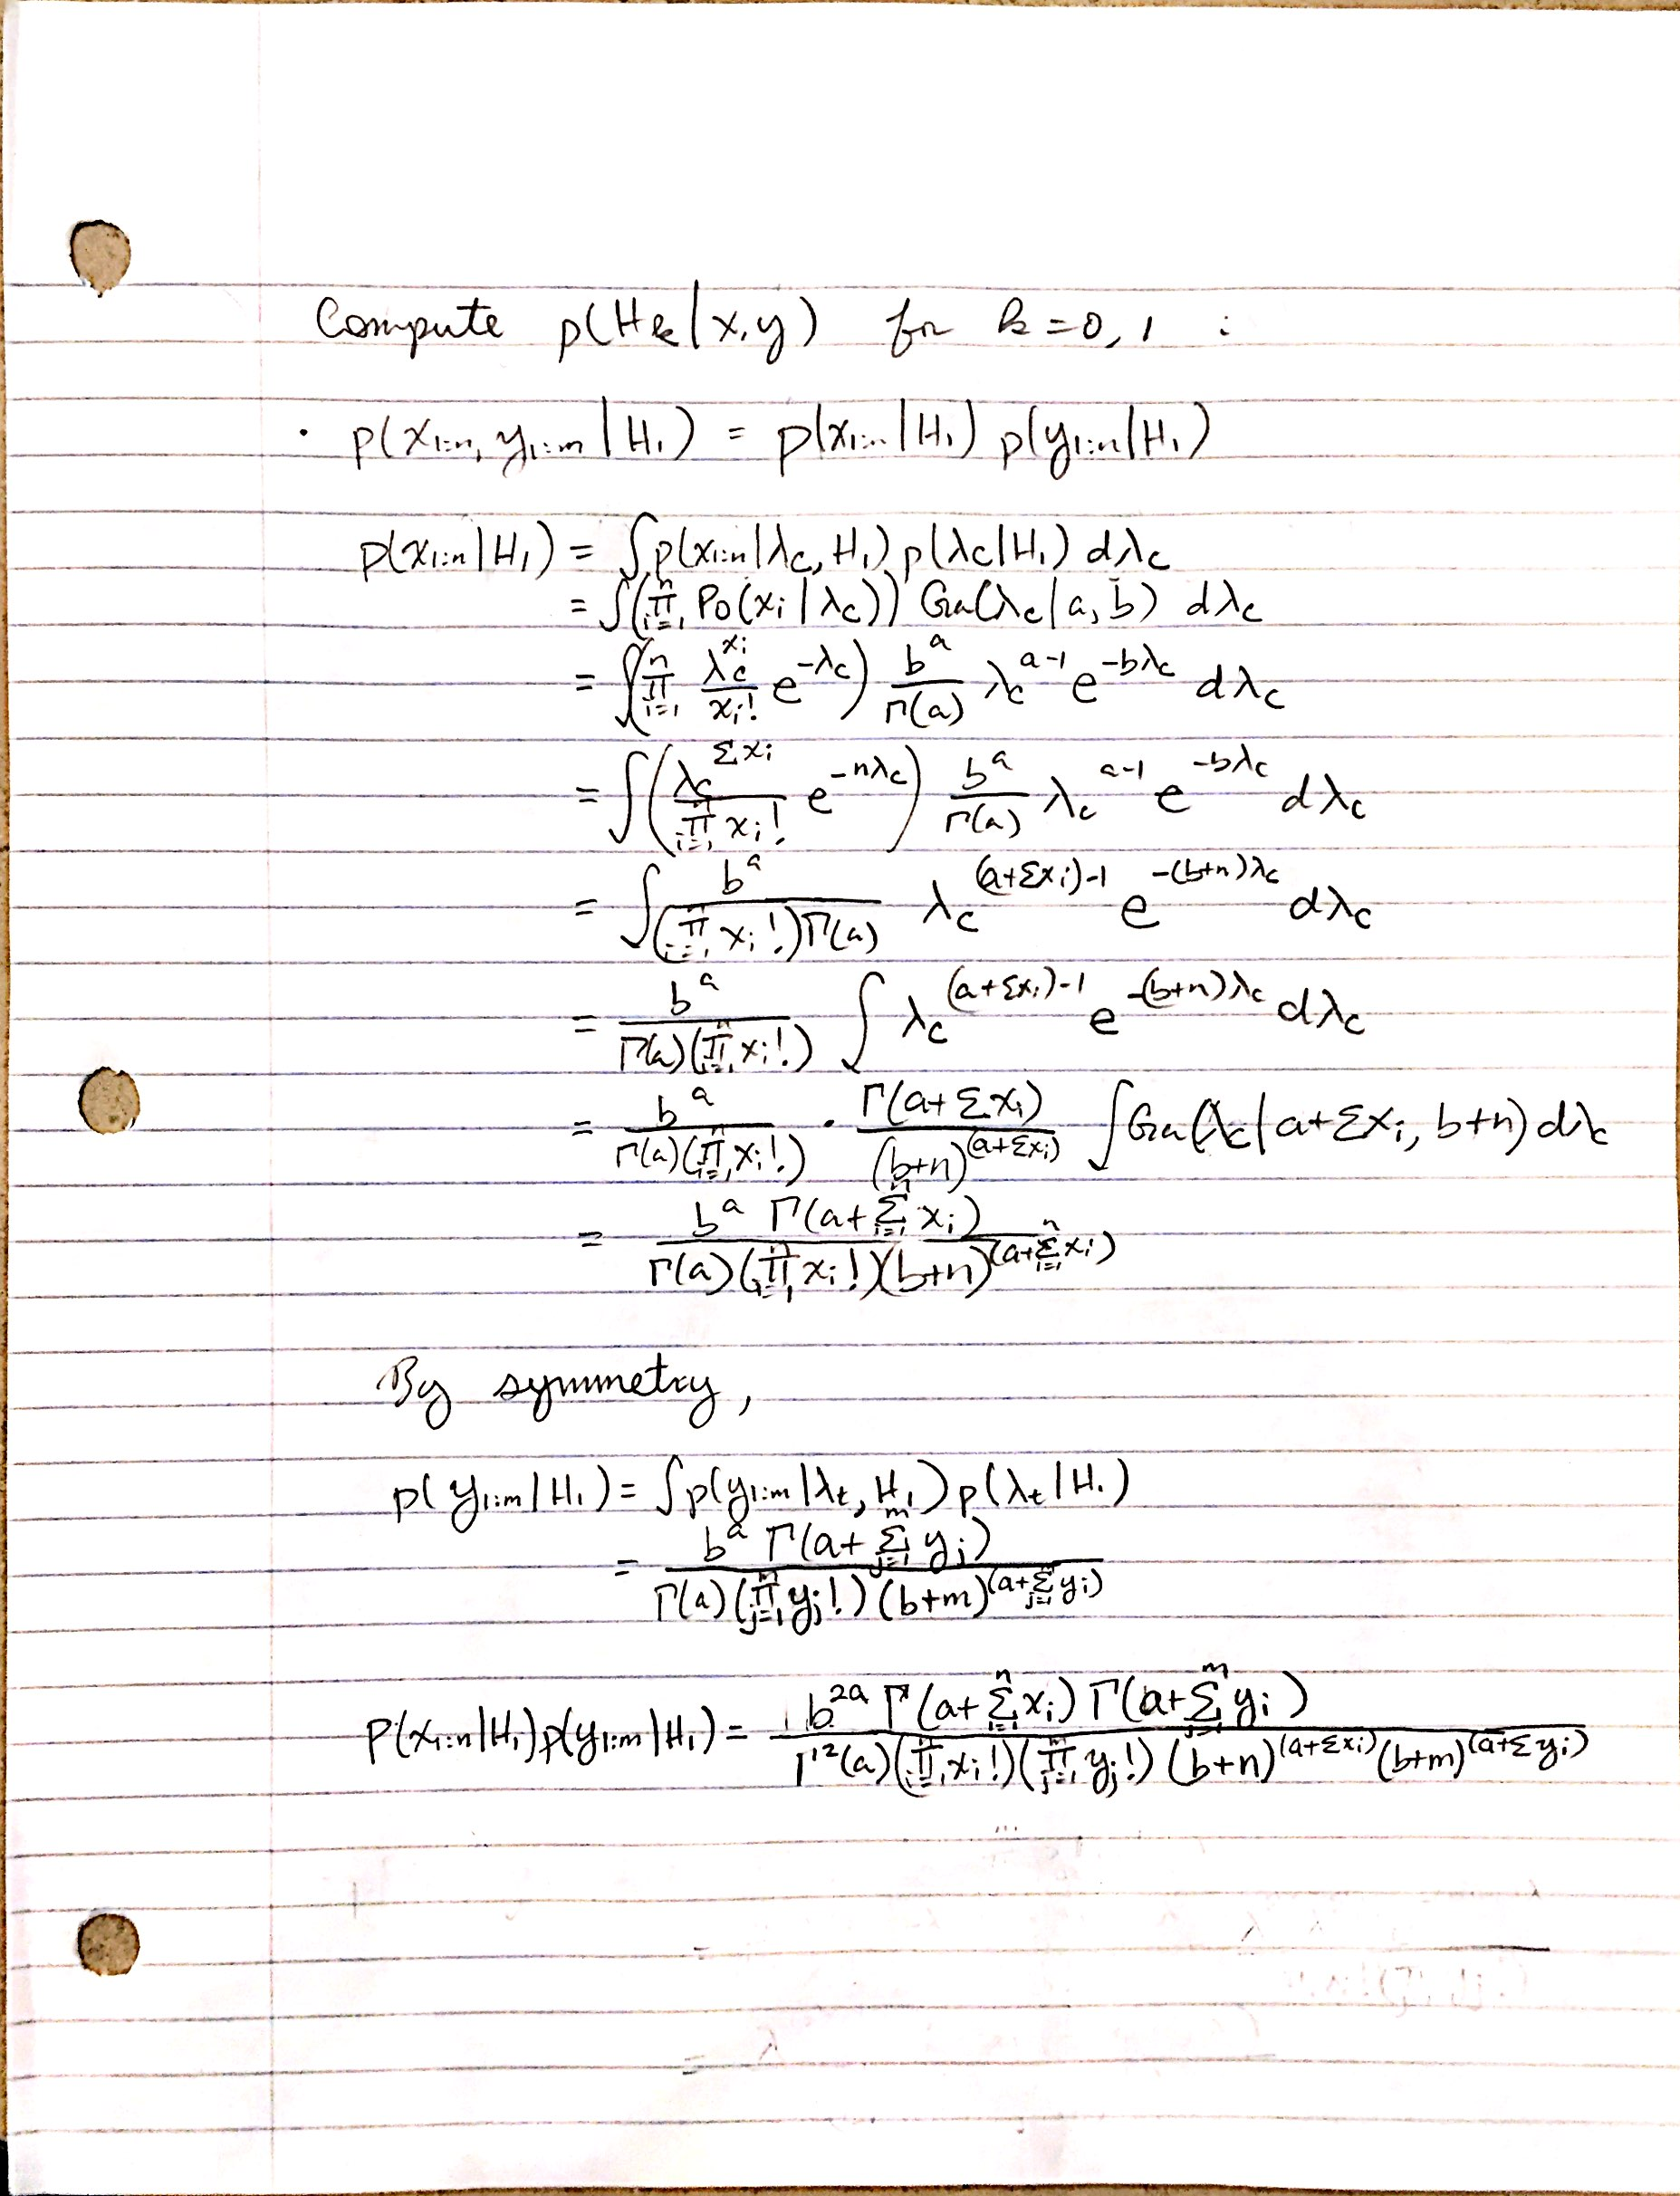
\includegraphics[scale = 0.23]{page1.jpg} \\
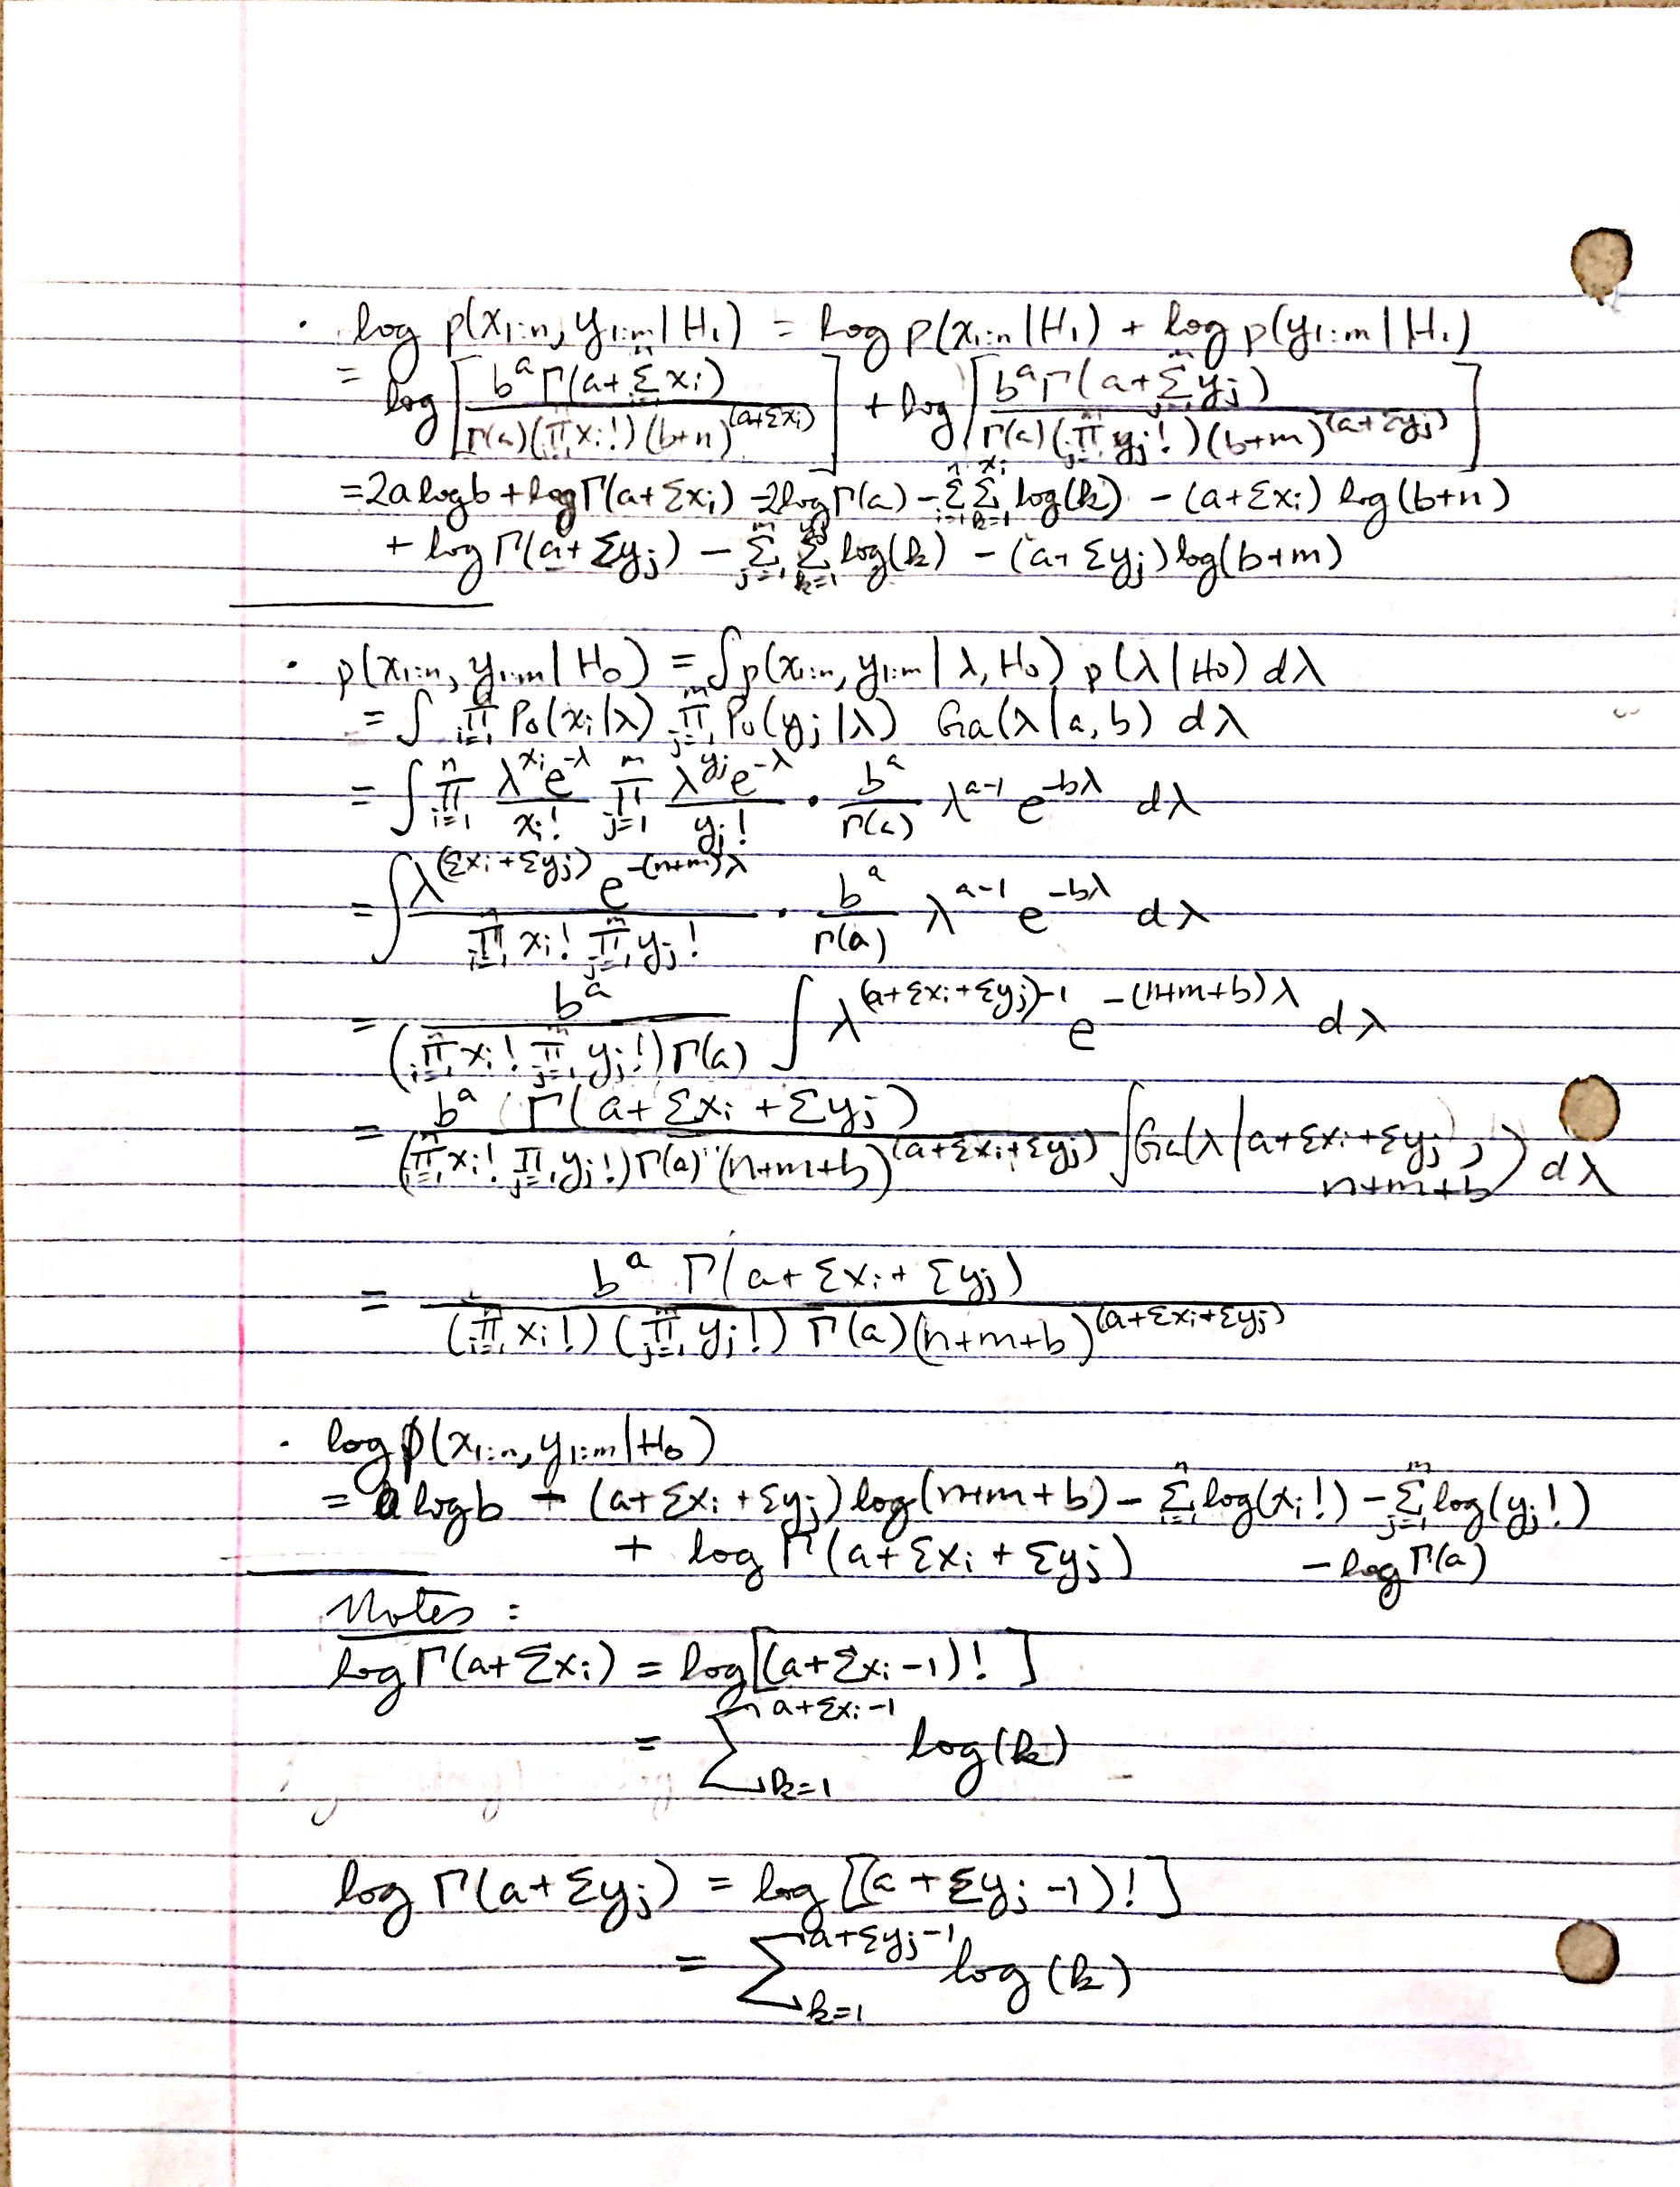
\includegraphics[scale = 0.23]{page2.jpg} \\
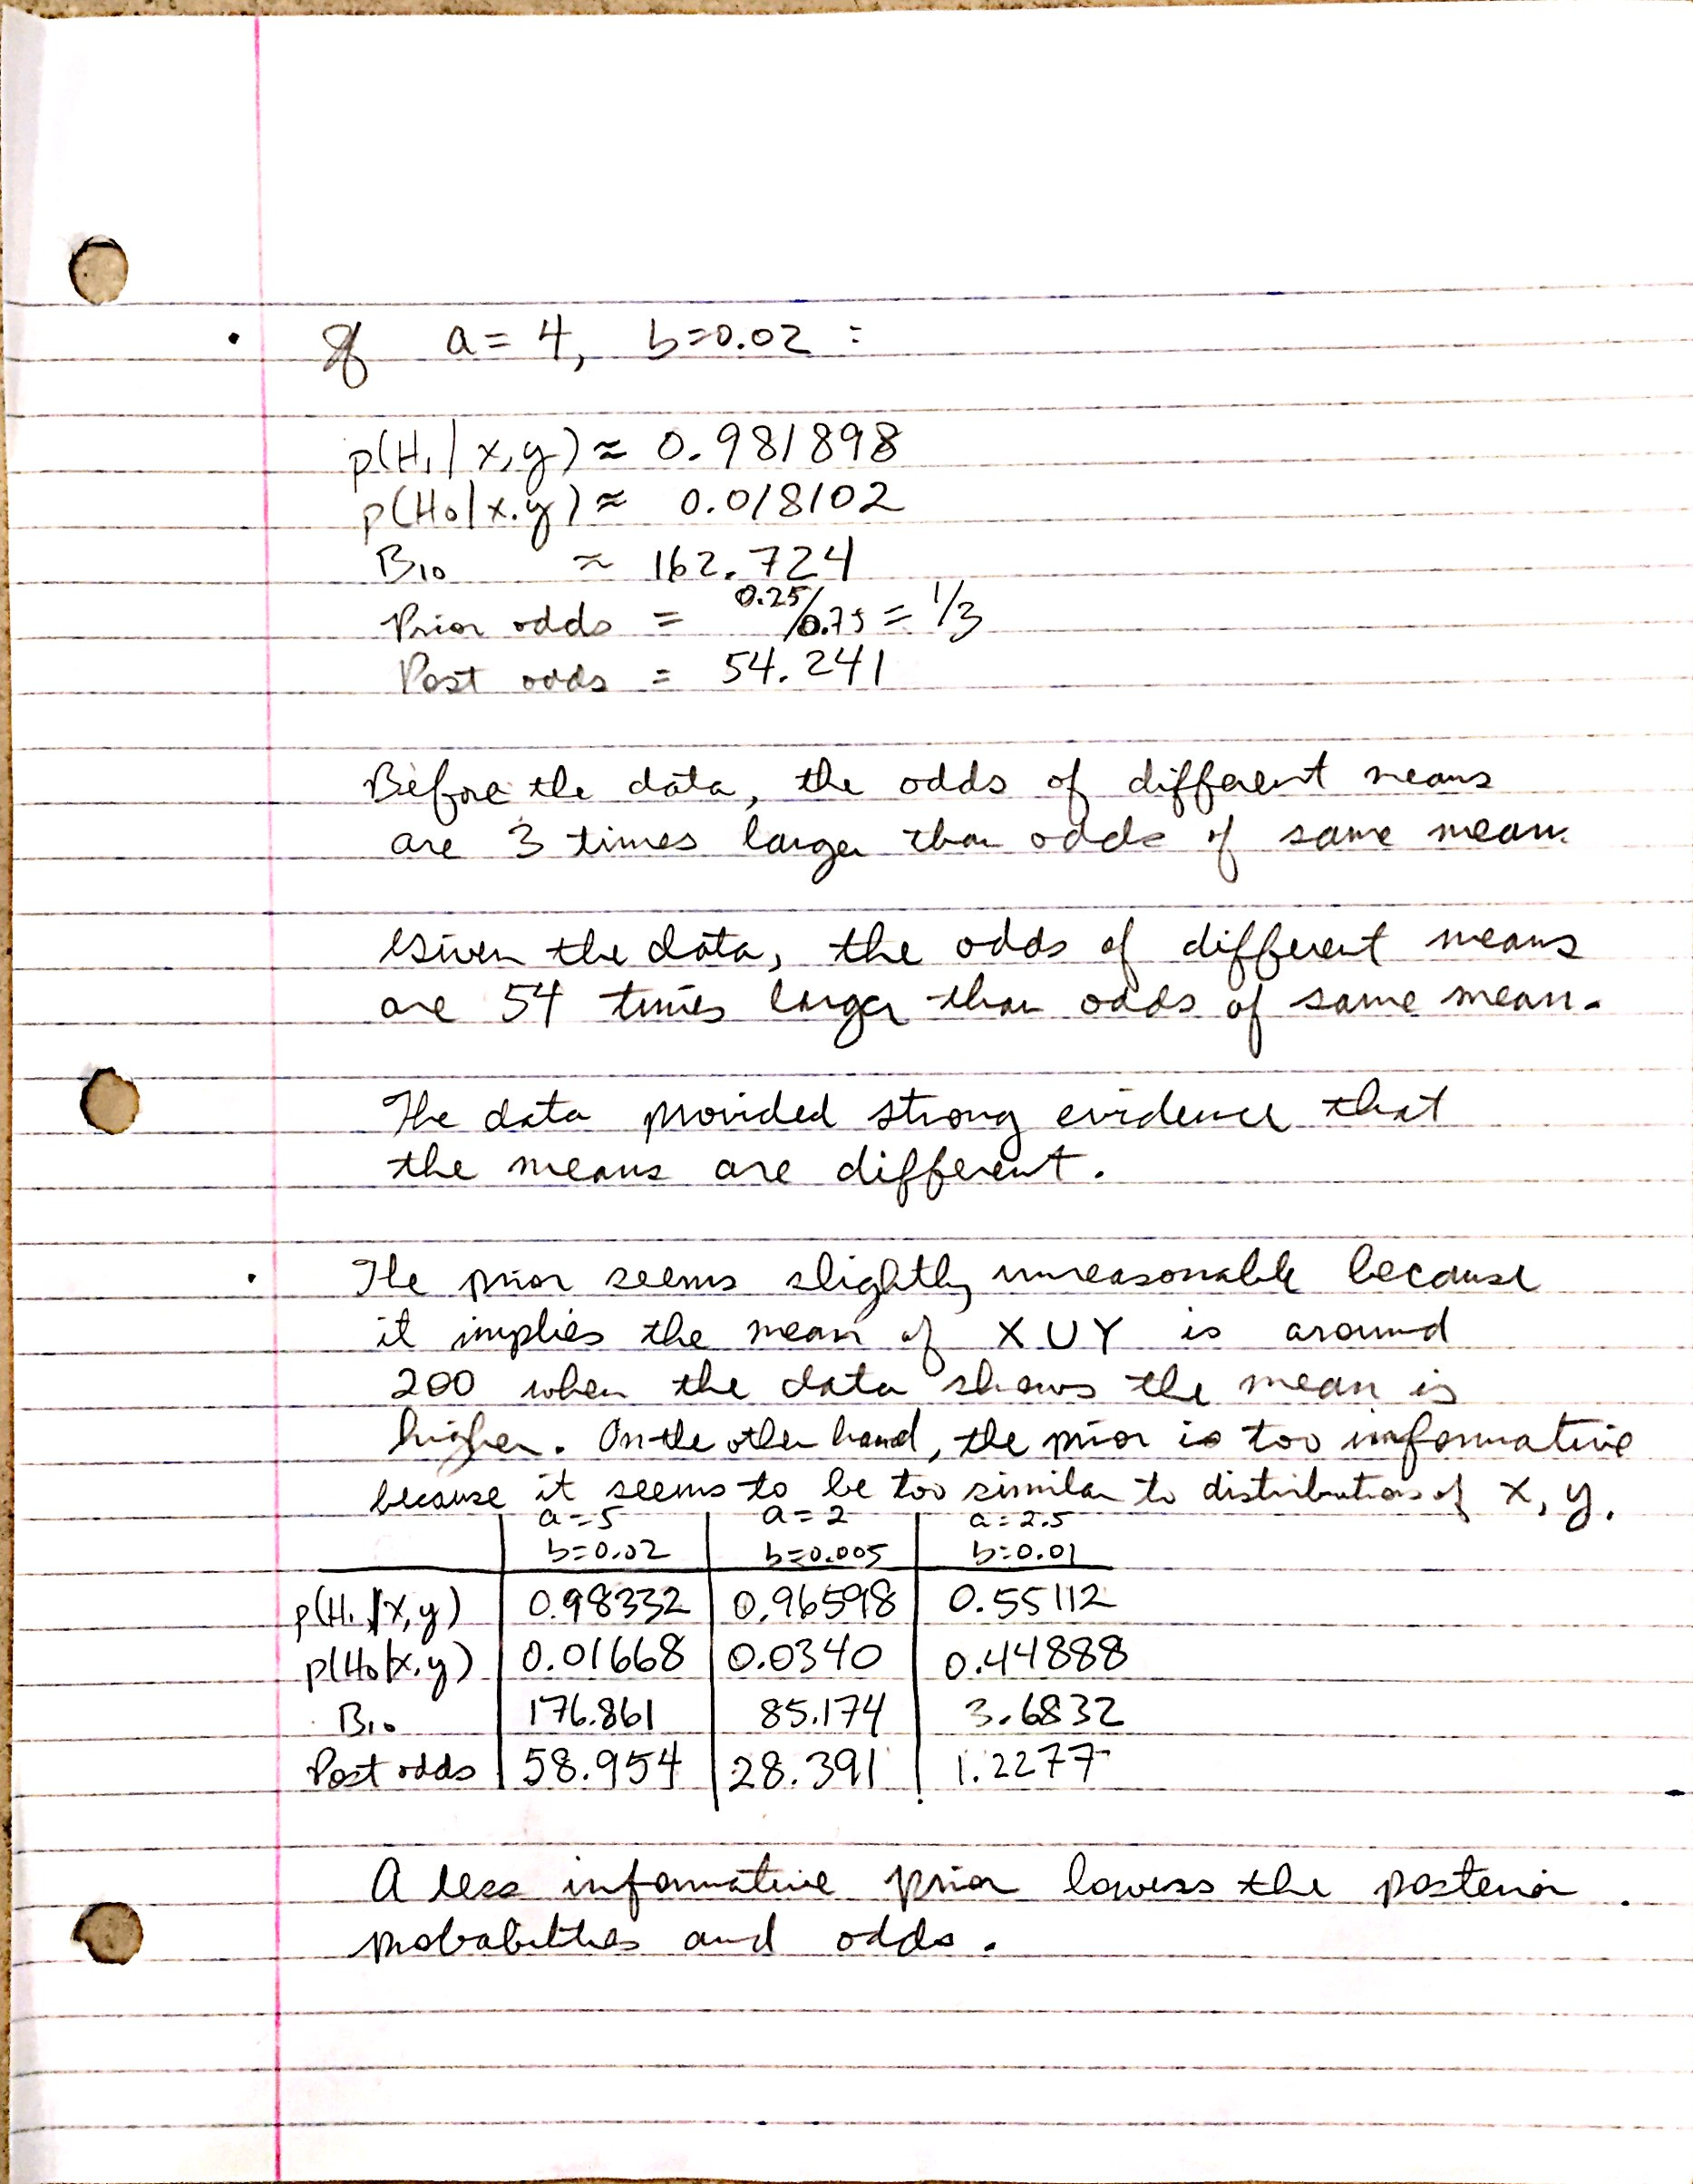
\includegraphics[scale = 0.23]{page3.jpg} \\

\pagebreak
R code for hypothesis testing:
\listinginput[1]{1}{cell.r}

\pagebreak
R code for 9.2:
\listinginput[1]{1}{diabetes.r}

\end{document}